\documentclass{standalone}
\usepackage{fontspec}
\setsansfont{DejaVuSans.ttf}[Path=./,Kerning=Off,Ligatures={TeXOff,NoCommon}]
\usepackage{tikz}
\begin{document}
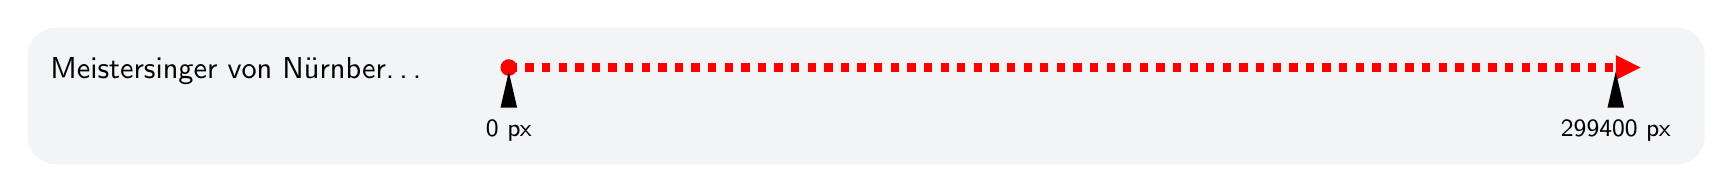
\begin{tikzpicture}[x=1pt,y=1pt,miter limit=4,font=\sffamily]
\definecolor{ts000000}{HTML}{000000}
\definecolor{tsF3F4F6}{HTML}{F3F4F6}
\definecolor{tsFF0000}{HTML}{FF0000}
\begin{scope}[shift={(16,16)}]
\path[rounded corners=10pt,fill=tsF3F4F6] (0,0) rectangle (605.9792,49.3789);
\path[draw=tsFF0000,line width=3pt,dash pattern=on 3pt off 3pt] (173.8511,34.9766) -- (573.8511,34.9766);
\path[fill=tsFF0000] (173.8511,34.9766) circle[radius=3];
\path[fill=tsFF0000] (582.8511,34.9766) -- (573.8511,39.4766) -- (573.8511,30.4766) -- cycle;
\path[fill=ts000000] (173.8511,33.4766) -- (170.8511,20.4766) -- (176.8511,20.4766) -- cycle;
\path[fill=ts000000] (573.8511,33.4766) -- (570.8511,20.4766) -- (576.8511,20.4766) -- cycle;
\node[anchor=base west,inner sep=0,font=\sffamily\fontsize{11}{12.8047}\selectfont,text=ts000000] at (8,31.1685) {Meistersinger von Nürnber…};
\node[anchor=base,inner sep=0,font=\sffamily\fontsize{9}{10.4766}\selectfont,text=ts000000] at (173.8511,10.1226) {0 px};
\node[anchor=base,inner sep=0,font=\sffamily\fontsize{9}{10.4766}\selectfont,text=ts000000] at (573.8511,10.1226) {299400 px};
\end{scope}
\end{tikzpicture}
\end{document}
